\subsection{Special case: ``soft'' K-means with Euclidean distances}

\begin{frame}{Turning Pairwise clustering into ``soft'' K-means}
Vectorial data: $\vec{x}^{(\alpha)}; \hspace{0.2cm} \alpha = 1,
\ldots, p; \hspace{0.2cm} \vec{x}^{(\alpha)} \in \mathbb{R}^N$,  Euclidean squared distances,
$$
	d_{\alpha \alpha^{'}} 
	= \frac{1}{2} \big( \vec{x}^{(\alpha)} - \vec{x}^{(\alpha^{'})}
		\big)^2
$$

Given the definition of prototypes in K-means:
\begin{equation}
	\vec{w}_q 
	= \frac{\sum\limits_{\gamma} \big< m_q^{(\gamma)} \big>_Q 
		\vec{x}^{(\gamma)}}{\sum\limits_{\gamma}
		\big< m_q^{(\gamma)} \big>_Q} 
\end{equation}

The mean fields can be expressed in terms of these prototypes:
\begin{equation}
	e_q^{(\alpha)} 
	= \frac{1}{2} \big( \vec{x}^{(\alpha)} - \vec{w}_q \big)^2
\end{equation}

\begin{itemize}
\itr center of mass of all objects weighted by their probability of assignment to cluster $q$
\end{itemize}

\end{frame}

% --------------------------------------------------------------------------
\begin{frame}[shrink=18]% \frametitle{Special case: ``soft'' K-means with Euclidean distances}
\begin{figure}[!th]
\footnotesize
\removelatexerror
\begin{algorithm}[H]
  \DontPrintSemicolon
  \textbf{Initialization:}\;
 - choose (maximum) number $M$ of partitions\; 
- choose initial ($\beta_0$) and final ($\beta_f$) values of the noise parameter\;
- initialize prototypes:  $\vec{w}_q = \frac{1}{p} 
\sum\limits_{\alpha} \vec{x}^{(\alpha)} + \vec{\eta}_q$ (small random vector)\;
- choose annealing factor $\eta$, convergence criterion $\theta$\;
- $\beta \leftarrow \beta_0$\;
  \While{$\beta < \beta_f$ (annealing)}{
\Repeat( EM){$\big| \vec{w}_q^{\mathrm{new}} - \vec{w}_q^{\mathrm{old}} \big| < \theta$ for all $q$}{
compute assignment probabilities: 
$ \big< m_q^{(\alpha)} \big>_Q = \frac{ \exp \big\{ -\frac{\beta}{2}
	\big( \vec{x}^{(\alpha)} - \vec{w}_q^{\mathrm{old}} \big)^2 \big\} }{
	\sum\limits_r \exp \big\{ -\frac{\beta}{2}
	\big( \vec{x}^{(\alpha)} - \vec{w}_r^{\mathrm{old}} \big)^2 \big\}}
	\hspace{0.1cm} \quad \forall \hspace{0.1cm} \alpha, q
$\;
\vspace{0.2cm}
compute new prototypes: \hspace{1.5cm} 
$ \vec{w}_q^{\mathrm{new}} \hspace{0.2cm}= \frac{\sum\limits_{\alpha} \big< 
	m_q^{(\alpha)} \big>_Q \vec{x}^{(\alpha)} }{
		\sum\limits_{\alpha} \big< m_q^{(\alpha)} \big>_Q}
		\hspace{0.1cm} \quad \forall \hspace{0.1cm} q
$

}  
$\beta \leftarrow \eta \beta$
}
\label{alg:softKmeansEuclidean}
\caption{Soft K-means clustering for Euclidean distances (batch version)}
\end{algorithm}
\end{figure}
\begin{block}{Interpretation}
\begin{itemize}
     \itl probabilistic cluster assignments.
	\itl natural extension of K-means clustering to the case of ``soft'' assignments
\end{itemize}
\end{block}
\end{frame}
% --------------------------------------------------------------------------

\subsection{Phase transitions in clustering}

%--------------------------------------------------------------------------
\begin{frame}[shrink=8] \frametitle{\subsecname}

\question{What are the implications of ``annealing'' in clustering (pairwise clustering, soft K-means)?}

Looking at average cost (Gibb's distribution of simulated annealing):
$$
	\big< E \big> = \frac{1}{Z} \sum\limits_{\big\{ m_p^{(\alpha)} \big\}}
	E \exp \big\{ -\beta E \big\}
$$

The annealing (i.e. increase of $\beta$) implies:
\begin{itemize}
  \item decrease of average cost 
  \item decrease of cluster size 
  \item increase in spatial resolution  (hierarchical clustering) - coarse to granular clustering
\end{itemize}

\end{frame}
% -----------------------------------------------------------------------

%--------------------------------------------------------------------------
\begin{frame} \frametitle{Summarizing overview}
\begin{center}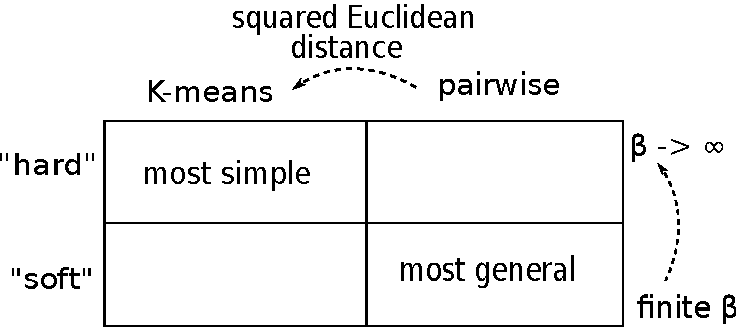
\includegraphics[scale=0.85]{img/section4_fig6a}
\end{center}
\begin{itemize}
%\item principled alternative to fuzzy clustering methods
	\itr mean-field annealing is robust against convergence to local optima
	\itr choice of terminal value of noise parameter $\beta \Rightarrow$ ``resolution''
		of cluster analysis
\end{itemize}
\end{frame}
